\chapter{Data Warehousing and Online Analytical Processing}
\clearpage

\section{Data Warehouse: Basic Concepts}
	
	\subsection{What Is a Data Warehouse?}

		Looseley speaking, a data warehouse refers to a data repository that is maintained
		seperately from organization's operational (ofen relational databases) databases. 

		\vspace{0.5cm}
		{\it \Large "A data warehouse is a subject-oriented, integrated, time-variant. and
		nonvolatile collection of data in support of management's decision making process."}
		\vspace{0.5cm}

		{\bf We will now look at the 4 key aspects of a data warehouse from the definition:}
		\begin{itemize}
			\item {\bf Subject-oriented:} a data warehouse is organized around major subjects
			such as customer, supplier, product and sales. Rather than concentrating on the 
			day-to-day operations and transaction processing of an organization, a data warehouse
			focuses on the modelling and analysis of data for decision makers. A data warehouse
			is a simple and concise view of particular subject issues by excluding data that 
			are not useful in the decision support process.
			\item{\bf Integrated:} A data warehouse is usually constructed by integrating
			multiple heterogeneous sources, such as relational databases, flat files, and online
			transaction records. Data cleaning and integration techniques are applied to ensure
			consistensy in naming convensions, encoding structures, attribute measures, and so on.
			\item {\bf Time-variant:} Data are stored to provide information from an historic 
			perspective. Every key structure in the data warehouse contains, either implicitly or
			explicitly, a time element.
			\item{\bf Nonvolatile ("flyktig"):} a data warehouse is always a physical seperate
			store of data transformed form the application data found in the operational environment.
			Due to this separation, a data warehouse does not require transaction processing, 
			recovery, and concurrency control mechanisms. It usually require only two operations
			in data accessing: {\it initial loading of data} and {\it access of data}.
		\end{itemize}

		{\bf How are organizations using information from data warehouses?} Many organizations
		use this information to support business decision-making activities, including:
		\begin{enumerate}
			\item Increasing customer focus, such as buying patterns (spending, time, interests, etc)
			\item Repositioning products and managing product portofolios by comparing 
			the perfomance of sales by quarter, year, and by geographic regions in order to 
			fine-tune production strategies. 
			\item Analyzing operations and looking for sources of profit.
			\item Managing customer relationships, making environmental corrections, and
			managing the cost of corporate aspects. 
		\end{enumerate}

		Data warehouseing is also very useful from the point of view of heterogeneous database
		integration. Organizations typically collect diverse kinds of data and maintain large
		databases from multiple, heterogeneous, autonomous, and distributed information sources. 
		It highly desirable, yet challenging, to integrate such data and provide easy and
		efficient access to it. 
	\clearpage

	\subsection{OLTP vs. OLAP}

		{\bf Online Transaction Processing (OLTP) systems:} \\
		The major task of online operational database systems is to perform online
		transaction and query processing. These systems are calles online transaction processing 
		(OLTP) systems. They cover most of the day-to-day operations of an organization
		such as purchasing, inventory, manufacturing, banking, payroll, egistration, and 
		accounting.

		{\bf Online Analytical Processing (OLAP) systems:} \\
		Data warehouse systems, on the other hand, serve users or knowledge workers in the role
		of data analysis and decision making. Such systems can organize and present data in 
		various formats in order to accommodate the diverse needs of different users. 
		These systems are known as online analytical processing (OLAP) systems. 

		{\bf Here are the major distinguishing features of OLTP and OLAP systems:}
		\begin{itemize}
			\item {\bf Users and system orientation:} An OLAP system is {\it customer-oriented}
			and is used for transaction and query processing. An OLAP system is {\it market-oriented}
			and is used for data analysis.
			\item {\bf Data contents:} OLTP are typically detailed data that is to complex in 
			decision making. An OLAP system manages large amount of histoic data, provides
			facilities for summaraization and aggregation, and stores and manages information 
			at different levels of granularity. These features make data easier to use for informed
			decision making. 
			\item {\bf Database design:} An OLTP system usually adopts an entity-relationship (ER)
			data model and an application oriented database design. An OLAP system typically adopts 
			either a star or snowflake model and a subject-oriented database design. 
			\item {\bf View:} An OLTP system focuses mainly on the current data within an enterprise
			or department, whitout referring to historic dataor data in different organization/sources.
			In contrast, an OLAP system often spans multiple versions of a database schema, due to 
			the evolutionary process of an organization. OLAP systems also deal with information 
			that organates from different organizations, integrating information from many data stores.
			Because of their huge volume, OLAP data are stored on multiple storage media. 
			\item {\bf Access patterns:} The access patterns of an OLTP system consist mainly of short, 
			atomic transactions. Such a system requires concurrency control and recovery mechanisms. 
			However, accesses to OLAP systems are mostly read-only  operations
			(becuase most data warehouses store historic rather than up-to-date information).
		\end{itemize}
	\clearpage
	\subsection{Why Have a Seperate Data Warehouse?}
		
		A major reason for separation is to help promote the {\bf high performance} of both systems
		because they have {\bf different usage situations}. Processing OLAP queries in operational
		databases would substantially degrade the performance of operational tasks. 

		Moreover, and operational database supports the concurrent processing of multiple
		transactions. {\bf Concurrancy control and recovery mechanisms} (e.g., locking and logging)
		are required to ensure the consistency and robustness of transactions. An OLAP
		query often needs read-only access of data records for summarization and aggegation,
		and therefore, the need of consistency and robustness is not the focus.
		Concurrancy and control and recovery mechanisms, if applied for such OLAP operations, 
		may jepardize the execution of concurrent transactions and thus substantially
		reduce the throughput of an OLAP system. 

		Finally, the separation of operational databases from data warehouses is based
		on the {\bf different structures}, contents, and uses of the data in these two systems. 

		Decision support requires consolidation (e.g., aggregation and summarization) of data
		from heterogeneous sources, resulting in {\bf high-quality, clean, integrated data}. In 
		contrast, operational databases contain only {\bf detailed raw data}, such as transactions, 
		which needs to be consolidated before analysis. 
		Because the two systems {\bf provide quite different functionalities and require different
		kinds of data}, it is presently necessary to maintain seperate databases. 

		\begin{figure}[H]
			\centering
			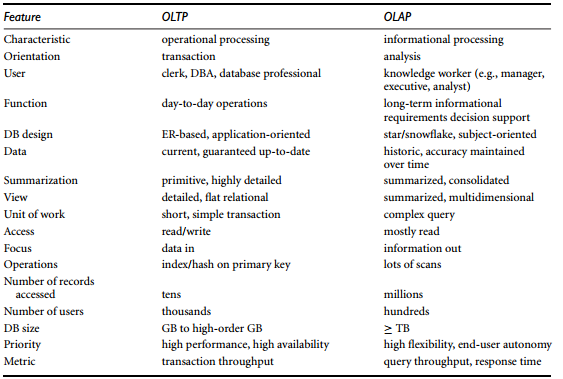
\includegraphics[width=\textwidth]{pics/oltpolap.png}
			\caption{OLTP vs. OLAP}
		\end{figure}

	\clearpage
	\subsection{Data Warehouse Multitier Architecture}

		{\bf "Tier 0" - Raw data:} this is not actually a layer in the data warehouse architecture, 
		but it is the collection of the raw data from operational databases and external sources.

		{\bf Tier 1 - Warehouse database servers:} is almost always a relational database system.
		Back-end tools and utilities are used to feed data into the bottom tier from operational
		databases or other external sources. These tools and utilities perform data extraction
		({\bf gateways}), 
		cleaning, and transformation (e.g., merge similar data from different sources into a 
		uniformed format), as well as load and refresh functions to update data warehouse. 

		{\bf Tier 2 - OLAP server:} typically implemented using either (1) a {\bf relational OLAP (ROLAP)}
		model; or (2) a {\bf multidimensional OLAP (MOLAP)} model. 

		{\bf Tier 3 - Front-end client layer:} contains query and reporting tools, analysis
		tools, and/or data mining tools.

		\begin{figure}[H]
			\centering
			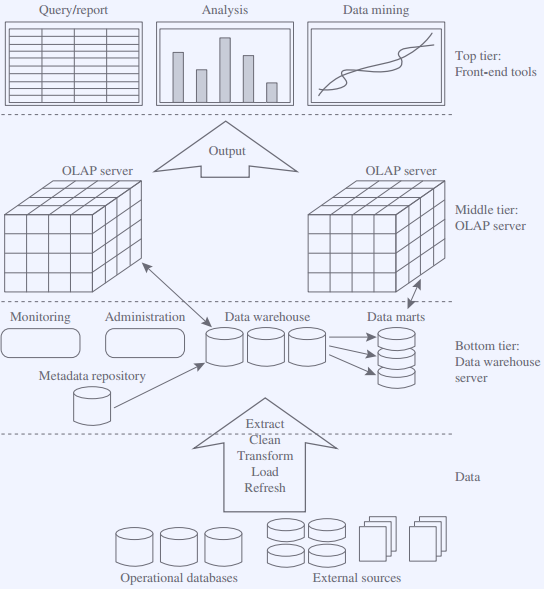
\includegraphics[width=\textwidth]{pics/mutitier.png}
		\end{figure}

	\clearpage
	\subsection{Data Warehouse Models}
		From the architecture point of view, there are three data warehouse models:

		{\bf Enterprise warehouse:} collects all information about subjects spanniing the
		entire organizaiton. It provides corporate-wide data integration, usually from
		one or more operational systems or external information providers, 
		and is cross-functional in scope. 

		{\bf Data mart:} contains subset of corporate-wide data that is one value to
		a specific group users. The scope is confined to specific selected subjects. 
		For example,  a marketing data mart confine its subjects to customer, item, and sales. 
		Depending on the source of data, data marts can be categorized as independent
		or dependent. Independent data marts are sourced from data captured from one
		or more operational systems or external infromation providers.
		Dependent data marts are sourced directly from enterprise data warehouses. 

		{\bf Virtual warehouse:} is a set of views over operational databases.
		For efficiency query processing, only some of the possible summary views may
		be materialized. A virtual warehouse is easy to build but requires excess capacity
		on operational database servers. 

		{\bf Top-down and bottom-up approaches to data warehouse development:}

		{\color{red} viktig ????}

	\subsection{Extraction, Transformation and Loading}

		Data warehouse systems use back-end tools and utilities to populate and refresh
		their data. These tools and utilities include the following functions:

			{\bf Data extraction:} tyically gathers data from multiple, heterogeneous,
			and external sources. 

			{\bf Data cleaning:} detects errors in the data and rectifies them when possible.
			
			{\bf Data transformation:} converts data from legacy or host format to warehouse
			format
			
			{\bf Load:} sort, summarizes, consolidates, computes views, checks integrity, and
			build indices and partitions. 
			
			{\bf Refresh:} propagates the updates from the data sources to the warehouse. 

	\subsection{Metadata Repository}

		{\bf Metadata} are data about data. When used in data warehouse, metadata are the
		data that define warehouse objects. Metadata in data warehouse are included in the
		bottom tire in the data warehousing architecture. A metadata repository should 
		contain the following:

			\begin{itemize}
				\item A description of the data warehouse structure
				\item Operational metadata
				\item The algorithms used for summarization
				\item Mapping from the operational environment to the data warehouse.
				\item Data related to system performance
				\item Business metadata, which include business terms and definitions, data
				ownership information, and charging policies.  
			\end{itemize}

\section{Data Warehouse Modelling: Data Cube and OLAP}
	
	Data warehouses and OLAP tools are based on a {\bf multidimentional data model}. This
	model views data in the form of a {\bf data cube}.
	
	\subsection{Data Cube: A Multidimensional Data Model}
		{\it What is a data cube?} A {\bf data cube} allows data to be modeled and viewed 
		in multiple dimensions. It is defined by dimensions and facts.

		In general terms, {\bf dimensions} are the perspectives or entities with repect to
		which an origanization wants to keep records. Each dimension may have a table 
		associated with it, called a {\bf dimension table}, which further describes the
		dimension. For example, a dimension table for item may contain the attributes
		item\_name, brand, and type. 

		A multidimensional data model is typically organized around a central theme, such
		as sales. This theme, is represented by a fact table. Facts are numeric measures.
		The {\bf fact table} contains the names of the facts, or measures, as well as keys
		to each of the related dimension tables.

		\begin{figure}[H]
			\centering
			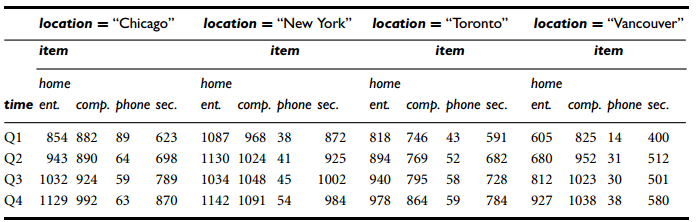
\includegraphics[scale=0.5]{pics/3D.png}
			\caption{3-D view of sales data according to time, item, and location}
		\end{figure}

		A cuboid is a way to represent multidimensional data. Given a set of dimensions, 
		The cuboid that holds the lowest level of summarization is called the {\bf base cuboid}.
		The first cuboid below is a nonbase cuboid because it summarizes for all suppliers. 
		\begin{figure}[H]
			\subfigure{
				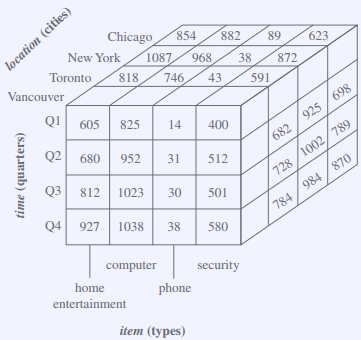
\includegraphics[scale=0.42]{pics/cuboid1.png}
			}
			\subfigure{
				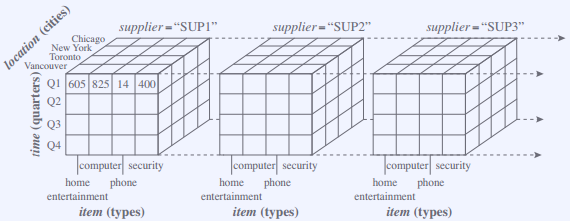
\includegraphics[scale=0.42]{pics/cuboid2.png}
			}
			\caption{Nonbase cuboid and base cuboid}
		\end{figure}

		\begin{figure}[H]
			\centering
			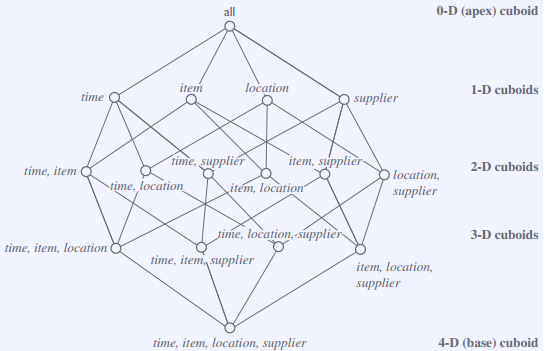
\includegraphics[scale=0.5]{pics/latticecuboid.png}
			\caption{Lattice of cuboids}
		\end{figure}

	\subsection{Stars, Snowflakes, and Fact Constellations}

		The entity-relationship (ER) data model is commonly used in the design of relational
		databses, where a database schema consists of a set of entities and the relationships
		between them.
		A data warehouse, however, requires a consise, subject-oriented schema that facilitates
		online data analysis. 

		The most popular data model for a data warehouse is a multidimensional model,
		which can exist in the for of a {\bf star schema}, a {\bf snowflake schema}, or
		a {\bf fact constellation schema}. 

		\subsection*{Star schema} 

		The most common modeling paradigm is the star schema, in which
		the data warehouse contains (1) a large central table ({\bf fact table}) containing
		the keys from all dimensions and other aggegated/summarization measures, and (2)
		a set of smaller attendant table ({\bf dimension tables}), one for each dimension.
		Notice that in the star schema, each dimension is represented by only one table, and
		each table contains a set of attributes. Since a dimension is only represented by one
		table, it can occur {\bf redundancy} since there is {\bf no normalization}. 

		\begin{figure}[H]
			\centering
				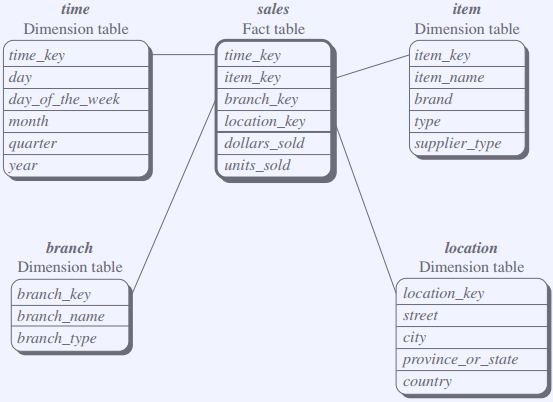
\includegraphics[scale=0.4]{pics/star.png}
				\caption{Star schema}
		\end{figure}

	\clearpage
		\subsection*{Snowflake schema} 

		The snowflake schema is a variant of the star schema model, where some dimension
		tables are normalized, therby further splitting the data into additional tables.
		The major difference between the showflake and the star schema models is that the
		dimension tables of the snowflake model may be kept in normalized form to reduce
		redundancies, but the snowflake structure can reduce the effeciveness of browsing, 
		since more joins will be needed to execute a query. 

		\begin{figure}[H]
			\centering
			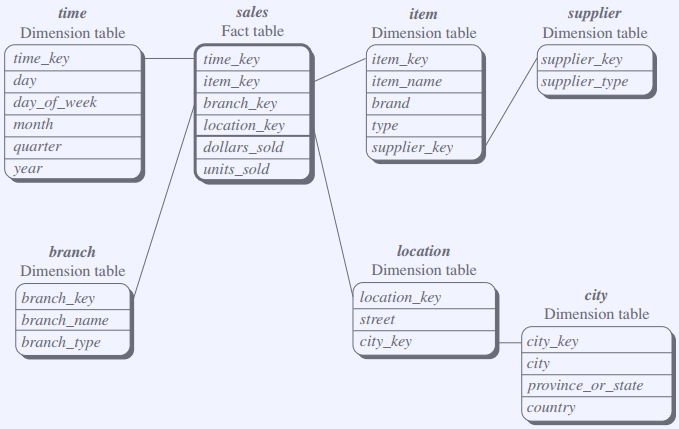
\includegraphics[scale=0.4]{pics/snowflake.png}
			\caption{Snowflake schema}
		\end{figure}

		\subsection*{Fact constellation/Galaxy schema}

		Applications may require multiple fact tabels to share dimensio tables. This kind of
		schema can be viewed as a collection of stars, and hence is called a {\bf galaxy schema}
		or a {\bf fact constellation}. A fact constillation schema allows dimension tables to
		be shared between fact tables. 

		\begin{figure}[H]
			\centering
			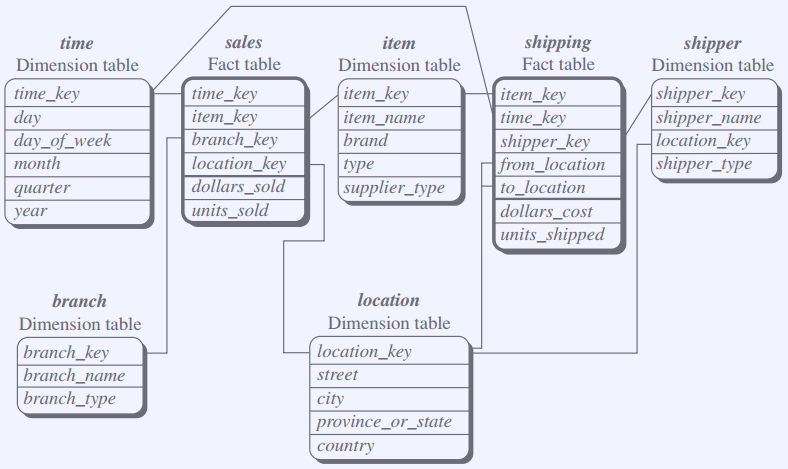
\includegraphics[scale=0.4]{pics/fact.png}
			\caption{Fact constellation/Galaxy schema with two fact tables}
		\end{figure}

		\clearpage
		\subsection*{The use of star, snowflake and galaxy schema}

		In data warehousing the is a distiction between a data warehouse and a data mart. 

		A {\bf data warehouse} collects information about
		subjects than span the {\bf entire organization}, such as customers, items, sales, 
		assets, and personnel, and thus its scope is {\bf enterprise wide.}
		For data warehouse, the fact {\bf constellation/galaxy} schema is commonly used, since it can model
		multiple, interrelated subjects. 

		A {\bf data mart}, on the other hand, is a department subset of the data warehouse that 
		focuses on selected subjects, and thus its scope is department-wide. For data marts, the
		{\bf star} or {\bf snowflake} schema is commonly used, since both are geared toward 
		modeling single subjects.


	\subsection{Dimensions - Concept Hierarchies}

		A {\bf concept hierarchy} defines a sequence of mappings from a set of low-level
		concepts to higher-level, more general concepts. We can look at this as a 
		ordering from high to low level. In the example below we have a {\bf total ordering}:
		country - province/state - city. 

		\begin{figure}[H]
			\centering
			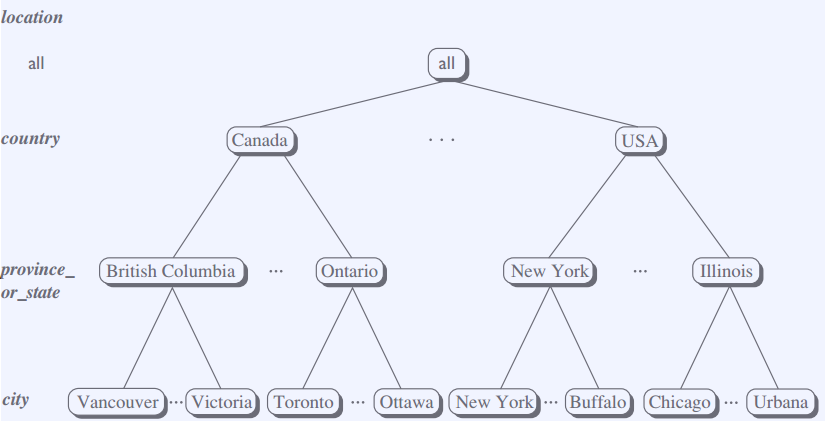
\includegraphics[scale=0.35]{pics/totalorder.png}
			\caption{Concept hierarchy (total order)}
		\end{figure}

		Alternatively, the attributes of a dimension may be organized as a {\bf partial order}, 
		forming a lattice. An example of a partial order for the time dimension based on 
		the attributs day, week, month, quarter, and year are shown below.

		A cencept hiearchy that is total or partial order among attributes in a database
		schema is called a {\bf schema hierarchy}.
		There may be more than one concept hierarchy for a given attribute or dimension., 
		based on different user viewpoints.  

		\begin{figure}[H]
			\centering
			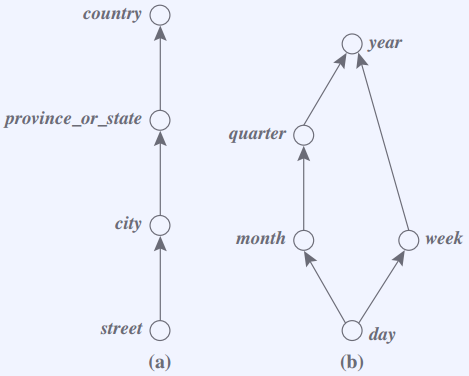
\includegraphics[scale=0.4]{pics/partialorder.png}
			\caption{Concept hierarchy (partial order)}
		\end{figure}

	\subsection{Measures}

		A data cube measure is a numeric function that can be evaluated at each point in the
		data cube space. 

		\subsection*{Distributive} 
		
		Suppose the data are partitioned into n sets. We apply a 
		function to each partition, resulting in n aggregate values. If the result
		derived by applying the function to the n aggregate values is the same as that 
		derived by applying the function to the entire data set, the function can be
		computed in a distributed manner. For example, sum() can be computed for 
		a data cube by first partitioning the cube into a set of subcubes, computing 
		sum() for each subcube, and then summing up the counts obtained for each subcube. 
		{\bf sum()}, {\bf min()}, and {\bf max()} is distributeive aggregate functions.

		A measure is distributive if it is obtained by applying a distributive aggregate
		function. 

		\subsection*{Algebraic} 

		An aggregate function is algebraic if it can be computed by an algebraic function
		with M aguments, each of which is obtained by applying a dristibutive aggregate function.
		For example, {\bf avg()} can be computed by sum()/count(), where both sum() and 
		count() are distributive aggregate functions. 
		{\bf min\_N()}, {\bf max\_N()}, {\bf avg()}, and {\bf standard\_deviation()} are all 
		algebraic aggregate functions. 

		\subsection*{Holistic}

		An aggregate function is  holistic if there is no constant bound on the storage
		size needed to describe a subaggregate. Common examples of holistic functions include
		{\bf median()}, {\bf mode()}, and {\bf rank()}.
		A measure is holistic if it is obtained by applying a holistic aggregate function. 

	\subsection{OLAP Operations}

		\subsection*{Roll-up}

			Performs aggregation on a data cube, either by climbing up a concept hierarchy
			for a dimension or by {\bf dimension reduction}. In the figure we see that the roll-up
			operation goes from city to the level of country (more abstraction).
			When roll-up is performed by dimension reduction, one or more dimensions are 
			removed from the given cube. 

		\subsection*{Drill-down}

			It navigates from less detailed data to more detailed data. Drill-down can be 
			realized by either stepping down a concept hierarchy for a dimension or 
			introducing additional dimensions. In the figure, the drill down goes from 
			quarters to month (detailed to more detailed). 

		\subsection*{Slice}

			The slice operation performs a selection on {\bf one dimension} of the given 
			cube, resulting in a subcube. The figure shows the slice operations by
			choosing time = Q1. 

		\subsection*{Dice}

			The dice operation defines a subcube by performing a selection on {\bf two or more
			dimensions}. In the figure, the dice operations chooses the following dimensions:
			location = "Toronto" or "Vancouver", time = "Q1" or "Q2", and
			item = "home entertainment" or "computer". 

		\subsection*{Pivot(rotate)}

			Pivot (also called rotate) is a visualization operation that rotates the data
			axes in view to provide an alternative data presentation. In the figure, show
			a pivot operation where item and location axes in a 2D slice are rotated. 
			Other examples include rotating the axes of a 3D cube, or transforming a 
			3D cube into a series of 2D plans. 

		\subsection*{Other OLAP operations}

			{\bf Drill-across} executes queries involving more than one fact table. 
			{\bf Drill-through} operations uses relational SQL facilities to drill
			through the bottom level of a cube down to its back-end relational tables. 

		\begin{figure}[H]	
			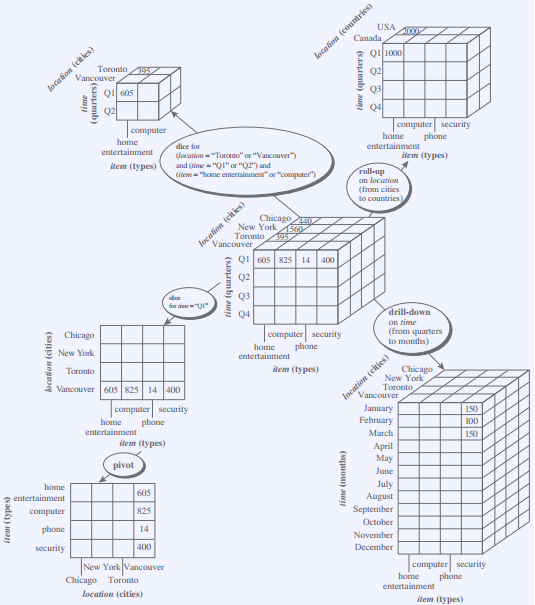
\includegraphics[width=\textwidth]{pics/operations.png}
		\end{figure}

\clearpage
\section{Data Warehouse Design and Usage}

	\subsection{Framework for Data Warehouse design}

		To design an effective data warehouse we need to understand and analyze
		business needs and construct  a business analysis framework. The construction
		of a large and complex building, for which the owner, architect, and builder
		have different views. These views are combined to form a complex framework 
		that represent top-down, business-driven, or owner's perspective, as 
		well as bottom-up, builder-driven, or implementor's view of the information system.

		Here are four different views regarding a data warehouse design:

		\begin{itemize}
			\item {\bf Top-down view} allows the selection of the relevant information
			necessary for the data warehouse. This information match current and 
			future business needs. 
			\item {\bf Data source point} exposes the information being captured, stored,
			and managed by operational systems. 
			\item {\bf Data warehouse view} includes fact tables and dimension tables. 
			\item {\bf Business query view} is the data perspective in the data warehouse
			from the end-user's viewpoint. 
		\end{itemize}

	\subsection{Data Warehouse Design Process}

		A data warehouse can be built using a top-down approach, a bottom-up approach,
		or a combination of both. 
		The {\bf top-down approach} starts with overall design and planning.
		It is useful in cases where the technology is mature and well known, and
		where the business problems that must be solved are clear and well understood.
		The {\bf bottom-up approach} starts with experiments and prototypes. 
		This is useful in the early stage of business modeling and technology development. 

		In general, the warehouse design process consists of the following steps:
		\begin{itemize}
			\item Choose a business process to model
			\item Chosse the business process gain
			\item Choose the dimensions that will apply to each fact table record
			\item Choose the measures that will populate each fact table record
		\end{itemize}

	\subsection{Data Warehouse Applications}

		There are three kind of data warehouse applications:
		\begin{itemize}
			\item {\bf Information processing:} supports querying, basic statistical analysis,
			and reporting using crosstabs, tables, charts or graphs.
			\item {\bf Analytical processing:} supports basic OLAP operations.
			\item {\bf Data mining:} supports knowledge discovery by finding hidden patterns
			and associations, constructing analytical models, performing classification 
			and prediction, and presenting the mining results using visualiization tools. 
		\end{itemize}

	\subsection{From OLAP to Multidimensional Data Mining}

		{\bf Multidimensional data mining} (also known as exploratory multidimensional data mining,
		{\bf online analytical mining (OLAM)}) integrates OLAP with data mining to 
		uncover knowledge in multidimensional databases. 

		Most data mining tools need to work on integrated, consistent, and cleaned data, which
		require costly data cleaning, data integration, and data transformation as
		{\bf preprocessing steps}. A data warehouse contains {\bf high quality (clean) data} that is ready
		to use for data mining, and there is no need for costly data cleaning in a 
		preprocessing step!

		Data warehoyse have an {\bf infrastructure} which connects different sources. It
		is prudent to make the best use of the available infrastructures rather than constructing
		everything from scratch. 

		Effective data mining need exploratory data analysis. A user will often want to traverse
		through a database, select portions of relevant data, analyze them, and present
		knowledge/results in different forms. This is a build in feature in data warehouse
		with OLAP operations as well as the visualisation possibilities of multidimensional data.

		

